\section{Handovers}
% handovers and research around it
Object handovers is a process that involves many parameters. Object grasping, timing of social cues and head gaze are just a few to mention some. Studies suggest that humans prefer a minimum jerk, human-like motion when being handed over an object \parencite{Huber2008} \parencite{Huber2008a}. As a consequence other research has set their focus on observing humans as to identify these parameters that affect a handover and their importance, with the aim of having robots immitate humans. \textcite{Moon2014} found that only by imitating human gaze cues during a handover the robot can help the human reach for the object sooner, even before the robot finishes the movement. \textcite{Huang2015} researched adaptation between humans in collaborative tasks, concluding that adaptevily coordinating actions can increase performance in tasks such as handovers between robots and humans. Although \textcite{Koene2014} found through their research that a fast motion from the robot was better recieved from the human side than a spatially accurate end position of the robotic grasp, \textcite{Admoni2014} showed through their experiments that introducing some deliberate delays in the handover help the reciever with focusing on the robot's head (i.e. gaze) and understand better it's suggestions which is proposed by \parencite{Moon2014}. However, the work of \textcite{Chan2015} found through a user study of handovers under different conditions that natural handovers may differ from reciever-oriented handovers, show us that robots would need to take this into account when learning from demonstration to make sure it puts the human interests in priority.

\begin{figure}
	\centering
	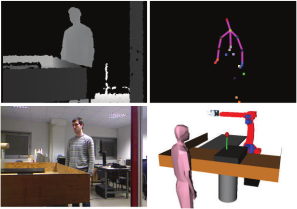
\includegraphics[width=0.5\textwidth]{img/related-work/planning-simulation.png}
	\caption{Human detection phase and handover planning in simulated environment in \parencite{Aleotti2012}}
\end{figure}

\section{Grasping}
% grasping
A very important feature as to insure the success of a handover, is the grasping of objects. Robotic grasping is itself a widely researched topic and several models have been proposed to compute proper grasping of objects. Some examples of previous work that attempt at defining the representation of the object and it's features for the task of grasping include \textcite{Miller2003} who decompose an object into primitive shapes to identify good grasping points (seen in figure \ref{fig:rel__shape-primitives}), while \textcite{Huebner2008} use a Minimum Volume Bounding Box solution to do the same. \textcite{Morales} represent objects by nine different high level descriptors of data and developed a learning framework upon this (seen in figure \ref{fig:rel__mvbb}). Just as with handovers, in the domain of grasping several studies have been conducted as to observe human grasping as to make robots immitate them. \parencite{Cutkosky1990} \parencite{Feix2009} \parencite{Kang1993} made taxonomies for different grasp choices used by humans depending on objects and tasks but seeing how force closures are usually quite limited in terms of mobility (at least relative to the humand hand), this thesis will not concentrate on the actual grasping and just leave it as future work after the correct grasping region has been identified as shown in figure \ref{fig:grasp-representation}. Please refer to the work in \parencite{Sahbani2012} for a complete review of the possibilities for robotic grasping. For the task of handovers, some research tried associating correct grasping of objects with their type and it's affordances (\parencite{Song2015}, \parencite{Chan2014}) where by associating an object with different ways of manipulating it we identify a grip which is best suited when handing it over as to increase productivity for the reciever.

\begin{figure}
	\centering
	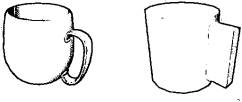
\includegraphics[width=0.3\textwidth]{img/related-work/shape-primitives.png}
	\caption{From \parencite{Miller2003}: A mug model and its primitive representation.}
	\label{fig:rel__shape-primitives}
\end{figure}

\begin{figure}
	\centering
	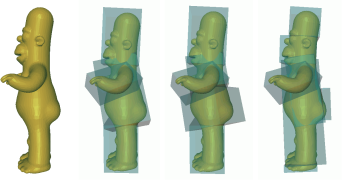
\includegraphics[width=0.5\textwidth]{img/related-work/mvbb.png}
	\caption{From \parencite{Huebner2008}: Minimum Volume Bounding Box on Homer model.}
	\label{fig:rel__mvbb}
\end{figure}

\begin{figure}
	\centering
	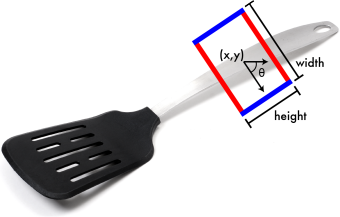
\includegraphics[width=0.3\textwidth]{img/related-work/grasp-representation.png}
	\caption{A five-dimensional grasp representation with terms of location, size and orientation. The blue lines demark the size and orientation of the gripper plates. The red lines show the approximate distance between the plates before the grasp is executed.}
	\label{fig:grasp-representation}
\end{figure}


\section{Machine-learned systems}
% rule based algorithms vs machine learning
Machine-learning systems have for a long a time been very limited in their ability to process raw natural data. Careful and intelligent preprocessing has been required as to transform this raw data into a smaller set of features that is easier for the machine to learn upon. This conversion is no easy task as it requires an expertise knowledge of the domain that the system is to be used within and can very time consuming to make sure it becomes correct. However, Deep learning systems through their large multi-layer setup are able to learn a hierarchy of features and are making large progress within machine-learned systems to perform representation learning from raw data, minimizing the amount of preprocessing to create the selected features \parencite{Lecun2015}. In the example of imagery, deep neural networks would learn how to extract global features such as edges from the image, and through the layers work on more complexe features within the patches extracted from the previous layer.

Convolutional Neural Networks (CNN) are a class of Artificial Neural Networks within deep learning that have a special architecture designed to process raw data that comes in multiple arrays such as the color channels in images which make them popular withing computer vision. CNNs are structured as a series of stages where the firsts ones are usually composed of layers of type convolutional and pooling, with the goal to detect local conjuctions of features from the previous layer (\parencite{Lecun2015}, \parencite{Jarrett2009}). With minimal preprocessing CNNs can learn a variety of high- and low-level features to perform with great accuracy several task within visual recognition. \textcite{Lee2009} demonstrate through unsupervised learning of a convolutional network how the network learns in the early layers edge detection and object parts. \textcite{Turaga2010} show by emphasizing the learning stage, they manage to train a CNN to learn edge detection with mininum pre- or postprocessing.

The perfomance of all types of ANNs is linked to their architecture. Changing the number of layers or their sizes can result in large fluctuations in performance, for the better or the worse. Some architectures become overtime more well-known for their success at certain tasks. One of them, named AlexNet, is the one published by \textcite{Krizhevsky2012} which achieved great results at the \textcite{ImageNet} image classification challenge ILSVRC-2012. In their work they credit the performance of their neural network to it's deep structure of many layers, showing that by only removing one of the convolutional layers it's performance would decrease of about 2\%. Figure \ref{fig:alexnet_orig} illustrates the network architecture of AlexNet.

\begin{figure}
	\centering
	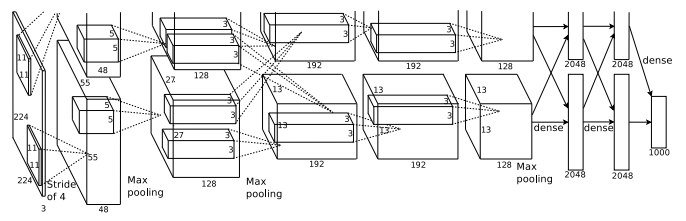
\includegraphics[width=\textwidth]{img/methods/alexnet_original.png}
	\caption{AlexNet architecture}
	\label{fig:alexnet_orig}
\end{figure}

Machine learned models are becoming more and more frequently used because of their high performance, they require less human intervention, as well as it has become increasingly easy to collect and represent data in a more versatile way. The works in \parencite{Aleotti2012} \parencite{Suay2015} \parencite{Kim2004} all report good results for handovers between robots and humans, but are supported by rule-based algorithms. Rule-based algorithms can present some limits of adaptation to a wider spectrum of scenarios than those thought of when the algorithm was created, they can as well become error prone because of human factors. \parencite{Redmon2014} \parencite{Lenz2015} \parencite{Jiang2011} \parencite{Huebner2008a} are examples of work that instead use the advantages of machine learned models to achieve good results, avoiding dictating the rules for grasping and handovers themselves. One disadvantage does nonetheless persist with these method, which is the fact that their datasets for training require the time consuming task of manually labeling.

\section{Autonomous learning}
\subsection{Learning by demonstration}
% learning from demonstration
% \textcite{Aleotti2012} developed a model based on user comfort for the reciever, in which the robot then scans environment and in a three dimensional reconstructed environment calculates the optimal handover by finding the best orientation of the object towards the human
% \textcite{Saxena2008} propose a solution for grasping new objects no longer needing complete 3D images, but the training phase nevertheless does so.
A less explored research field is yet to teach robots grasping and handovers by demonstrations. Having robots learn by observing humans would enable faster collection of data, save time from manually labeling and allow the robot to use more human-like motions. Common within robot simulation is that the data required for processing is represented by 3D models of the objects and environment (for example in \parencite{Miller2003}) which are not trivial to come by for newly encountered objects in a live setting as it would require the robot to see everything from all angles. Another factor is the accuracy of sensors and quality control of the data (i.e was it as good handover?) are some of the limitations of learning from observations which makes it a challenging method. Kinect sensors have become popular within robotics today because of their relatively low cost and support for depth data which can help in creating three dimensional renderings of images. \parencite{Lenz2015} \parencite{Redmon2014} \parencite{Jiang2011} \parencite{Saxena2008} are example of works that propose methods for training and identifying grasp sites using RGBD images recorded by a stereo camera, but the problem with these works is that they do not train on data collected by demonstrations without manual annotation. \textcite{Chan2014} collected data by observing humans interacting with objects, but the data covered other scenarios of object interaction than handovers. \textcite{Strabala2013} trained a model using decision trees from recorded data of humans performing handovers, but they had to manually label the recorded material with eye-gaze, two-dimensional position of participants, object locations and handover positions. \textcite{Chan2015a} do however propose a framework for robots to learn handovers and grasp sites through demonstration. By handing objects to a robot they then have the robot repeat the handover in reverse order back to the human. They however do not have the robot learn any object features as to associate the handover features to it that can be used on previously untrained objects.

% new objects
\subsection{Foreign objects}
One of the challenges within robotic grasping and handovers is the ability to perform their task on an object that the robot has never seen nor been trained for. Some previous research do enable grasping of foreign objects, but requires a lot of data which itself needs to be labeled. For example \textcite{Huebner2008a} in a continuation of their work in \parencite{Huebner2008}, train a neural network that can be used for grasping of novel objects, but requires the network to be trained on a previously manually labeled dataset of grasps. Also the proposed model by \parencite{Chan2014} requires data on different ways to manipulate an object before the robot can calculate a way of grasping it and handing it over, making it hard to deploy in a new environment. Complete and accurate 3D models are unfortunately not always available and not feasible in an environment where a robot should learn from observing humans.

\begin{figure}
	\centering
	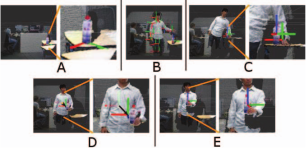
\includegraphics[width=\textwidth]{img/related-work/demonstrations.png}
	\caption{From \parencite{Chan2015a}: Stages of extracting grasp configurations from handover demonstrations. A - Object detection. B - Human detection and tracking. C - Grasp point detection. D - Direction of torso-to-hand vector for handover cue detection. E - Object orientation at handover.}
\end{figure}

% how to use this related work for this thesis
\textcite{Redmon2014} show very promising results with their implementation in finding grasp sites on objects, even for those that are not present in the training set, illustrating the high performance of convolutional neural networks. Their work is based on the ImageNet model that was further trained with RGBD images for detecting grasp regions. The ImageNet model is however trained for RGB images, the authors solved this by dropping the blue channel and replacing it with the depth data. In figure \ref{fig:rel__cnn-arch} we can find an overview of their full architecture for their network. The problem is that the data that it needs for training is manually annoted. The framework proposed in \parencite{Chan2015a} is a good starting point for the collection of data as to train a model that can be later used for grasping and handovers. This thesis will try and combine these works by implementing a framework for collecting data through demonstration from humans and process it as to train a convolutional neural network that can later identify grasping sites and handover features on novel objects through RGBD images.

\begin{figure}
	\centering
	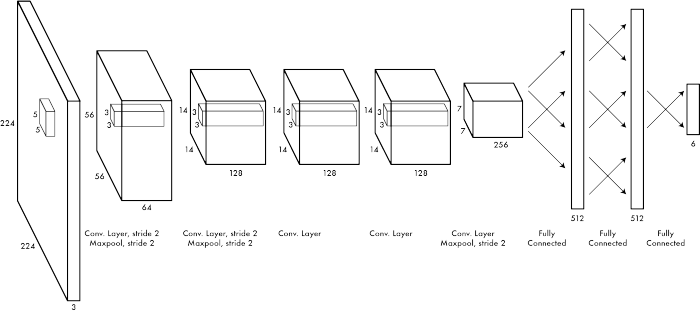
\includegraphics[width=\textwidth]{img/related-work/cnn-architecture.png}
	\caption{Full architecture used by \textcite{Redmon2014}.}
	\label{fig:rel__cnn-arch}
\end{figure}
